%!TEX root = ../thesis.tex

\chapter{中国东南部深对流对痕量气体垂直分布的影响}

\section{模式设置}

\subsection{气象及化学设置}

该研究使用的WRF-Chem版本号为4.1.4,气象条件的初始场和边界场来自1小时分辨率的欧洲中心大气再分析数据(ERA5,\citet{Hersbach.2020})。
模式的垂直分层为75层,对流层顶设置为50 hPa,嵌套区域如图\ref{fig:domains_china}所示。
微物理过程使用WSM6方案\citep{Hong.2006a},而短波和长波辐射使用RRTMG方案\citep{Iacono.2008},陆面过程由Noah方案模拟\citep{Koren.1999}。
但是,我们使用不同的边界层参数化来模拟两次对流个例,2019年的个例使用YSU方案\citep{Hong.2006},而2020年的个例使用QNSE方案\citep{Sukoriansky.2005}。
闪电部分未使用参数化,用闪电同化代替,详见\ref{sect:lightning_assimilation}节。

化学初始场和边界场采用整个大气社区气候模型(WACCM,\url{https://www.acom.ucar.edu/waccm/})的输出数据。
其中2020年个例的初始O$_3$廓线使用臭氧探空仪观测所得的O$_3$廓线。
人为排放使用2016年中国多分辨率排放清单 (MEIC,\url{http://www.meicmodel.org/})1.3版驱动,生物排放采用来自自然界的气体和气溶胶排放模型(MEGAN;\citet{Guenther.2006})。
化学机理使用气相化学的臭氧和相关化学示踪剂模式(MOZART)和气溶胶的Goddard化学气溶胶辐射和传输(GOCART)模式\citep{Pfister.2011}。
其中光解方案采用基于云光学厚度(cloud\_fraction$^{1.5}$)的新 TUV(对流层紫外线和可见光)方案,即光解速率依赖于气溶胶和云。
此外,LNO的垂直廓线使用\citet{Ott.2010}的双峰型闪电NO(LNO)廓线\citep{Laughner.2017},而LNO和LNO$_2$廓线是指开启和关闭闪电选项的模拟之间垂直廓线的差异。
其中LNO$_x$参数化调整为每次闪电产生500 mol NO\citep{Zhu.2019}。

\begin{figure}[htbp]
\centering
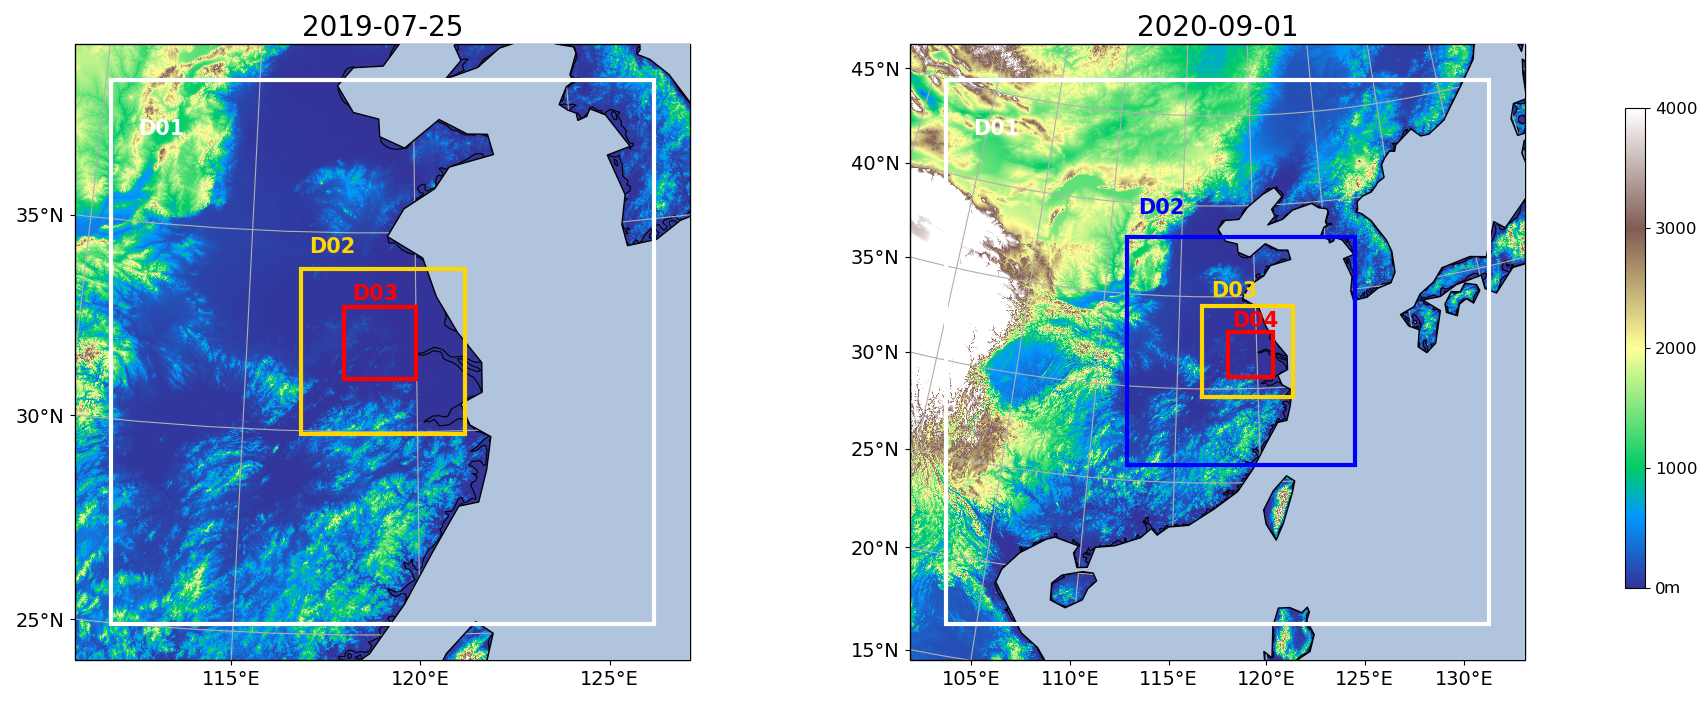
\includegraphics[width=0.9\textwidth]{./figures/domains_china.png}
\caption{2019年和2020年个例的WRF-Chem模拟区域和地形高度(m)图。
2019年个例的水平网格分辨率为15 km(D01)、3 km(D02)和 0.6 km(D03)。
对于2020年个例,分别为27 km(D01)、9 km(D02)、3 km(D03)和 1 km(D04)。\\
Figure \ref{fig:domains_china}. Domain and terrain height (m) of the WRF-Chem simulations for the 2019 and 2020 cases. The horizontal grid resolution of
domains for the 2019 case is 15 km (D01), 3 km (D02) and 0.6 km (D03). For the 2020 case, it is 27 km (D01), 9 km (D02), 3 km (D03),
and 1 km (D04).}
\label{fig:domains_china}
\end{figure}

\subsection{闪电同化} \label{sect:lightning_assimilation}

为了更准确地模拟出对流和LNO$_x$,我们将闪电数据同化应用于 WRF-Chem。
闪电数据同化方法详见\citet{Fierro.2012}和\citet{Li.2017b},主要步骤为在发生闪电所处网格的垂直恒温层间,增加水汽质量混合比。

\begin{equation} \label{eq:lda}
Q_{v}=A Q_{\mathrm{sat}}+B Q_{\mathrm{sat}} \tanh (C X)\left[1-\tanh \left(D Q_{g}^{\alpha}\right)\right]
\end{equation}

式(\ref{eq:lda})中,Q$_{sat}$ 为水汽饱和混合比(g kg$^{−1}$),Q$_g$为霰粒混合比(g kg$^{−1}$),X 为闪电频率。
本研究选择263.15 和 290.15 K作为恒温层的上下界限,其目的是为了让对流在行星边界层中快速扎根,因为对流层低层的Q$_v$更深\citep{Marchand.2014,Finney.2016,Li.2017b}。
参数设置参考\citet{Li.2017b}:A=0.94,B=0.2,C=0.001,D=0.25,α=2.2。
其中网格化的总闪数据通过WRF的辅助输入流进行每10分钟的读取。
例如,如果闪电同化开始于05:00 UTC,时间步长为10 min,则将05:00--05:10 UTC之间特定网格中所有闪电数相加作为此期间的贡献。
在下一个时间步长,闪电被归类为下一个新组。
因此,闪电数即闪电频率的密度(单位:flash每10 min 每dx km 每dy km),其中dx和dy分别是模型网格在x和y方向的分辨率。
如\citet{Fierro.2012}和\citet{Li.2017b}所述,这可以确保所有嵌套层中的闪电密度相同。
此外,闪电数也被直接同化进WRF-Chem中,该方法已被应用于社区多尺度空气质量(CMAQ,\citet{Kang.2019,Kang.2019a,Kang.2020}模式中。

\section{模式评估}

与雷达观测相比,2019年7月25日和2020年9月1日模拟的对流初生时间,较实际情况分别提前了60分钟和30分钟(图\ref{fig:comp_crf_2019}和图\ref{fig:comp_crf_2020}),闪电数据也以相同的时间间隔提前同化。
对于下文的结果比较,我们选择匹配的阶段而不是相同的时间。

2019年7月25日的热对流在初始时呈现为孤立的热泡,WRF-Chem再现了初始阶段孤立对流的位置和强度(图\ref{fig:comp_crf_2019}a和\ref{fig:comp_crf_2020}d)。
在05:40 UTC时,对流系统呈现东北-西南向,最大组合雷达反射率达到60 dBZ(图\ref{fig:comp_crf_2019}b),强度大于模拟的对流(最大组合雷达反射率为55 dBZ,图\ref{fig:comp_crf_2019}e)。
将模拟的对流核心区的雷达反射率垂直剖面与观测结果进行比较(图\ref{fig:comp_dbzcross_2019}),
虽然对流与雷达距离过远造成缺失数据较多,但是在未进行人工插值的条件下,孤立对流的水平和垂直结构仍大致显示。
模拟的45 dBZ等值线达到12 km,但由于10 km 以上的数据质量低,观测到的等值线仅达到10 km。

2020年9月1日观测到的飑线在北部初生,然后加强,并向观测点移动(图\ref{fig:comp_crf_2020})。
对流旺盛阶段(最大组合雷达反射率为60 dBZ)大致在05:50 UTC,与TROPOMI过境时间相符(图\ref{fig:comp_dbzcross_2020}b和e)。
虽然该飙线抵达的最高高度低于2019年的热对流,但对流层低层(2--8 km)的反射率更大更广(图\ref{fig:comp_dbzcross_2020})。
由于模拟的对流消散区偏离了雷达观测到的消散区,这导致与臭氧探空仪比较的区域设置在站店的西边(图\ref{fig:comp_dbzcross_2020}c和f)。

在不同对流阶段测量的O$_3$和Q$_v$分布如图\ref{fig:ozonesonde_profile}所示。
一般来说,对流导致上对流层O$_3$和Q$_v$浓度增大,且增强的最大值所在区域为10--16 km 之间。
然而,2020年的个例观测显示对流层低层(2--8 km)的O$_3$有较大的增加。
此外,两个个例都存在双谷形状的O$_3$剖面,但高度不同:2019年的热对流个例为2 km和8 km,2020年的飑线为4 km和10 km。
尽管WRF-Chem模型倾向于分别低估2019年和2020年的下对流层和上对流层中的O$_3$浓度,但它可以再现详细的O$_3$垂直分布结构,故能用以分析对流影响O$_3$的机制。
共有三个可能的来源可以解释上对流层中O$_3$的增加:对流输送、化学反应和闪电直接产生的O$_3$。
本研究仅详细讨论了前两个因素,因为闪电直接产生的O$_3$超出了本研究的范围并且有限的观测和模式模拟所示其产量仍不确定\citep{Morris.2010,Ripoll.2014}。


\begin{figure}[htbp]
\centering
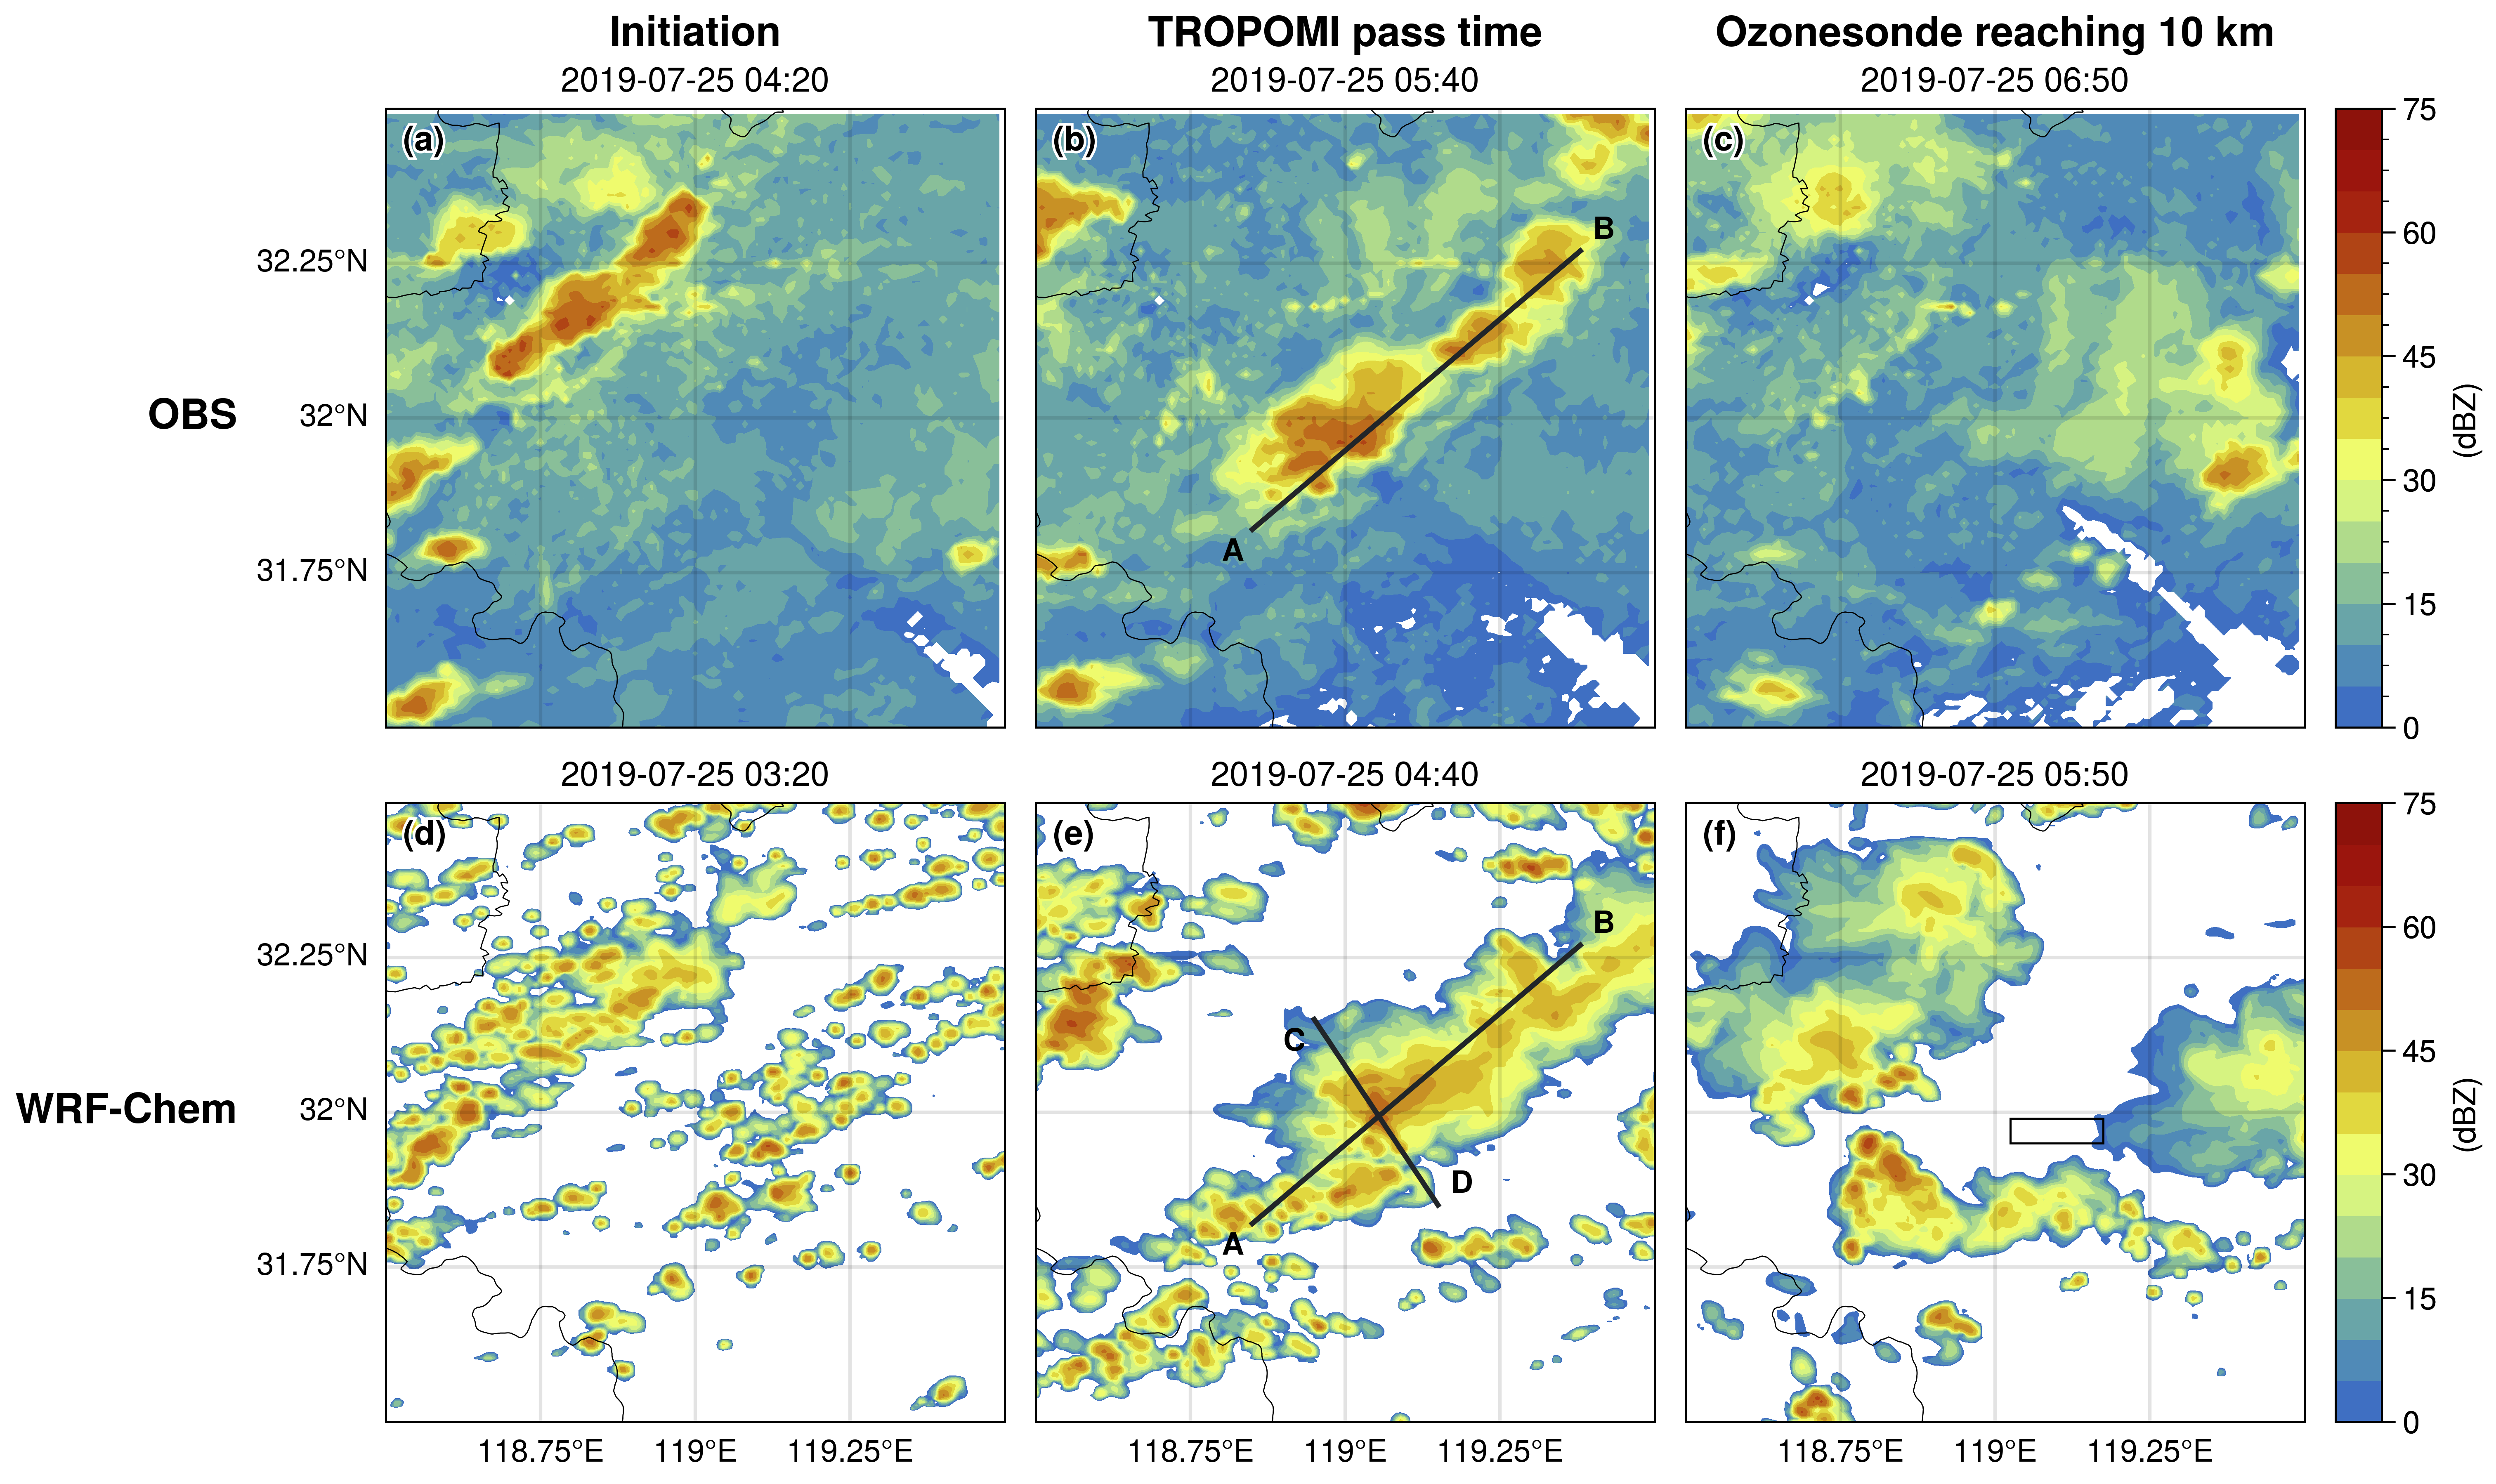
\includegraphics[width=0.9\textwidth]{./figures/comp_crf_2019.png}
\caption{在 (a) 04:20 UTC、(b) 05:40 UTC 和 (c) 06:50 UTC 观测到的雷达组合反射率。
         (d--e) WRF-Chem 在雷达观测时间前一小时模拟的雷达组合反射率。
         (b) 和 (e) 中的 AB 实线是图 \ref{fig:comp_dbzcross_2019} 的剖面线。
         (e)中的CD实线是图\ref{fig:tendency_o3}b的剖面线。
         黑色矩形是与臭氧探空仪进行比较的区域。\\
Figure \ref{fig:comp_crf_2019} Observed radar composite reflectivity at (a) 04:20 UTC, (b) 05:40 UTC, and (c) 06:50 UTC.
        (d--e) WRF-Chem simulated composite reflectivity one hour before the radar observation times.
        The AB solid lines in (b) and (e) are cross section lines for Fig. \ref{fig:comp_dbzcross_2019}.
        The CD solid line in (e) is the cross section line for Fig. \ref{fig:tendency_o3}b.
        The black rectangle is the region for the comparison with ozonesonde.}
\label{fig:comp_crf_2019}
\end{figure}

\begin{figure}[htbp]
\centering
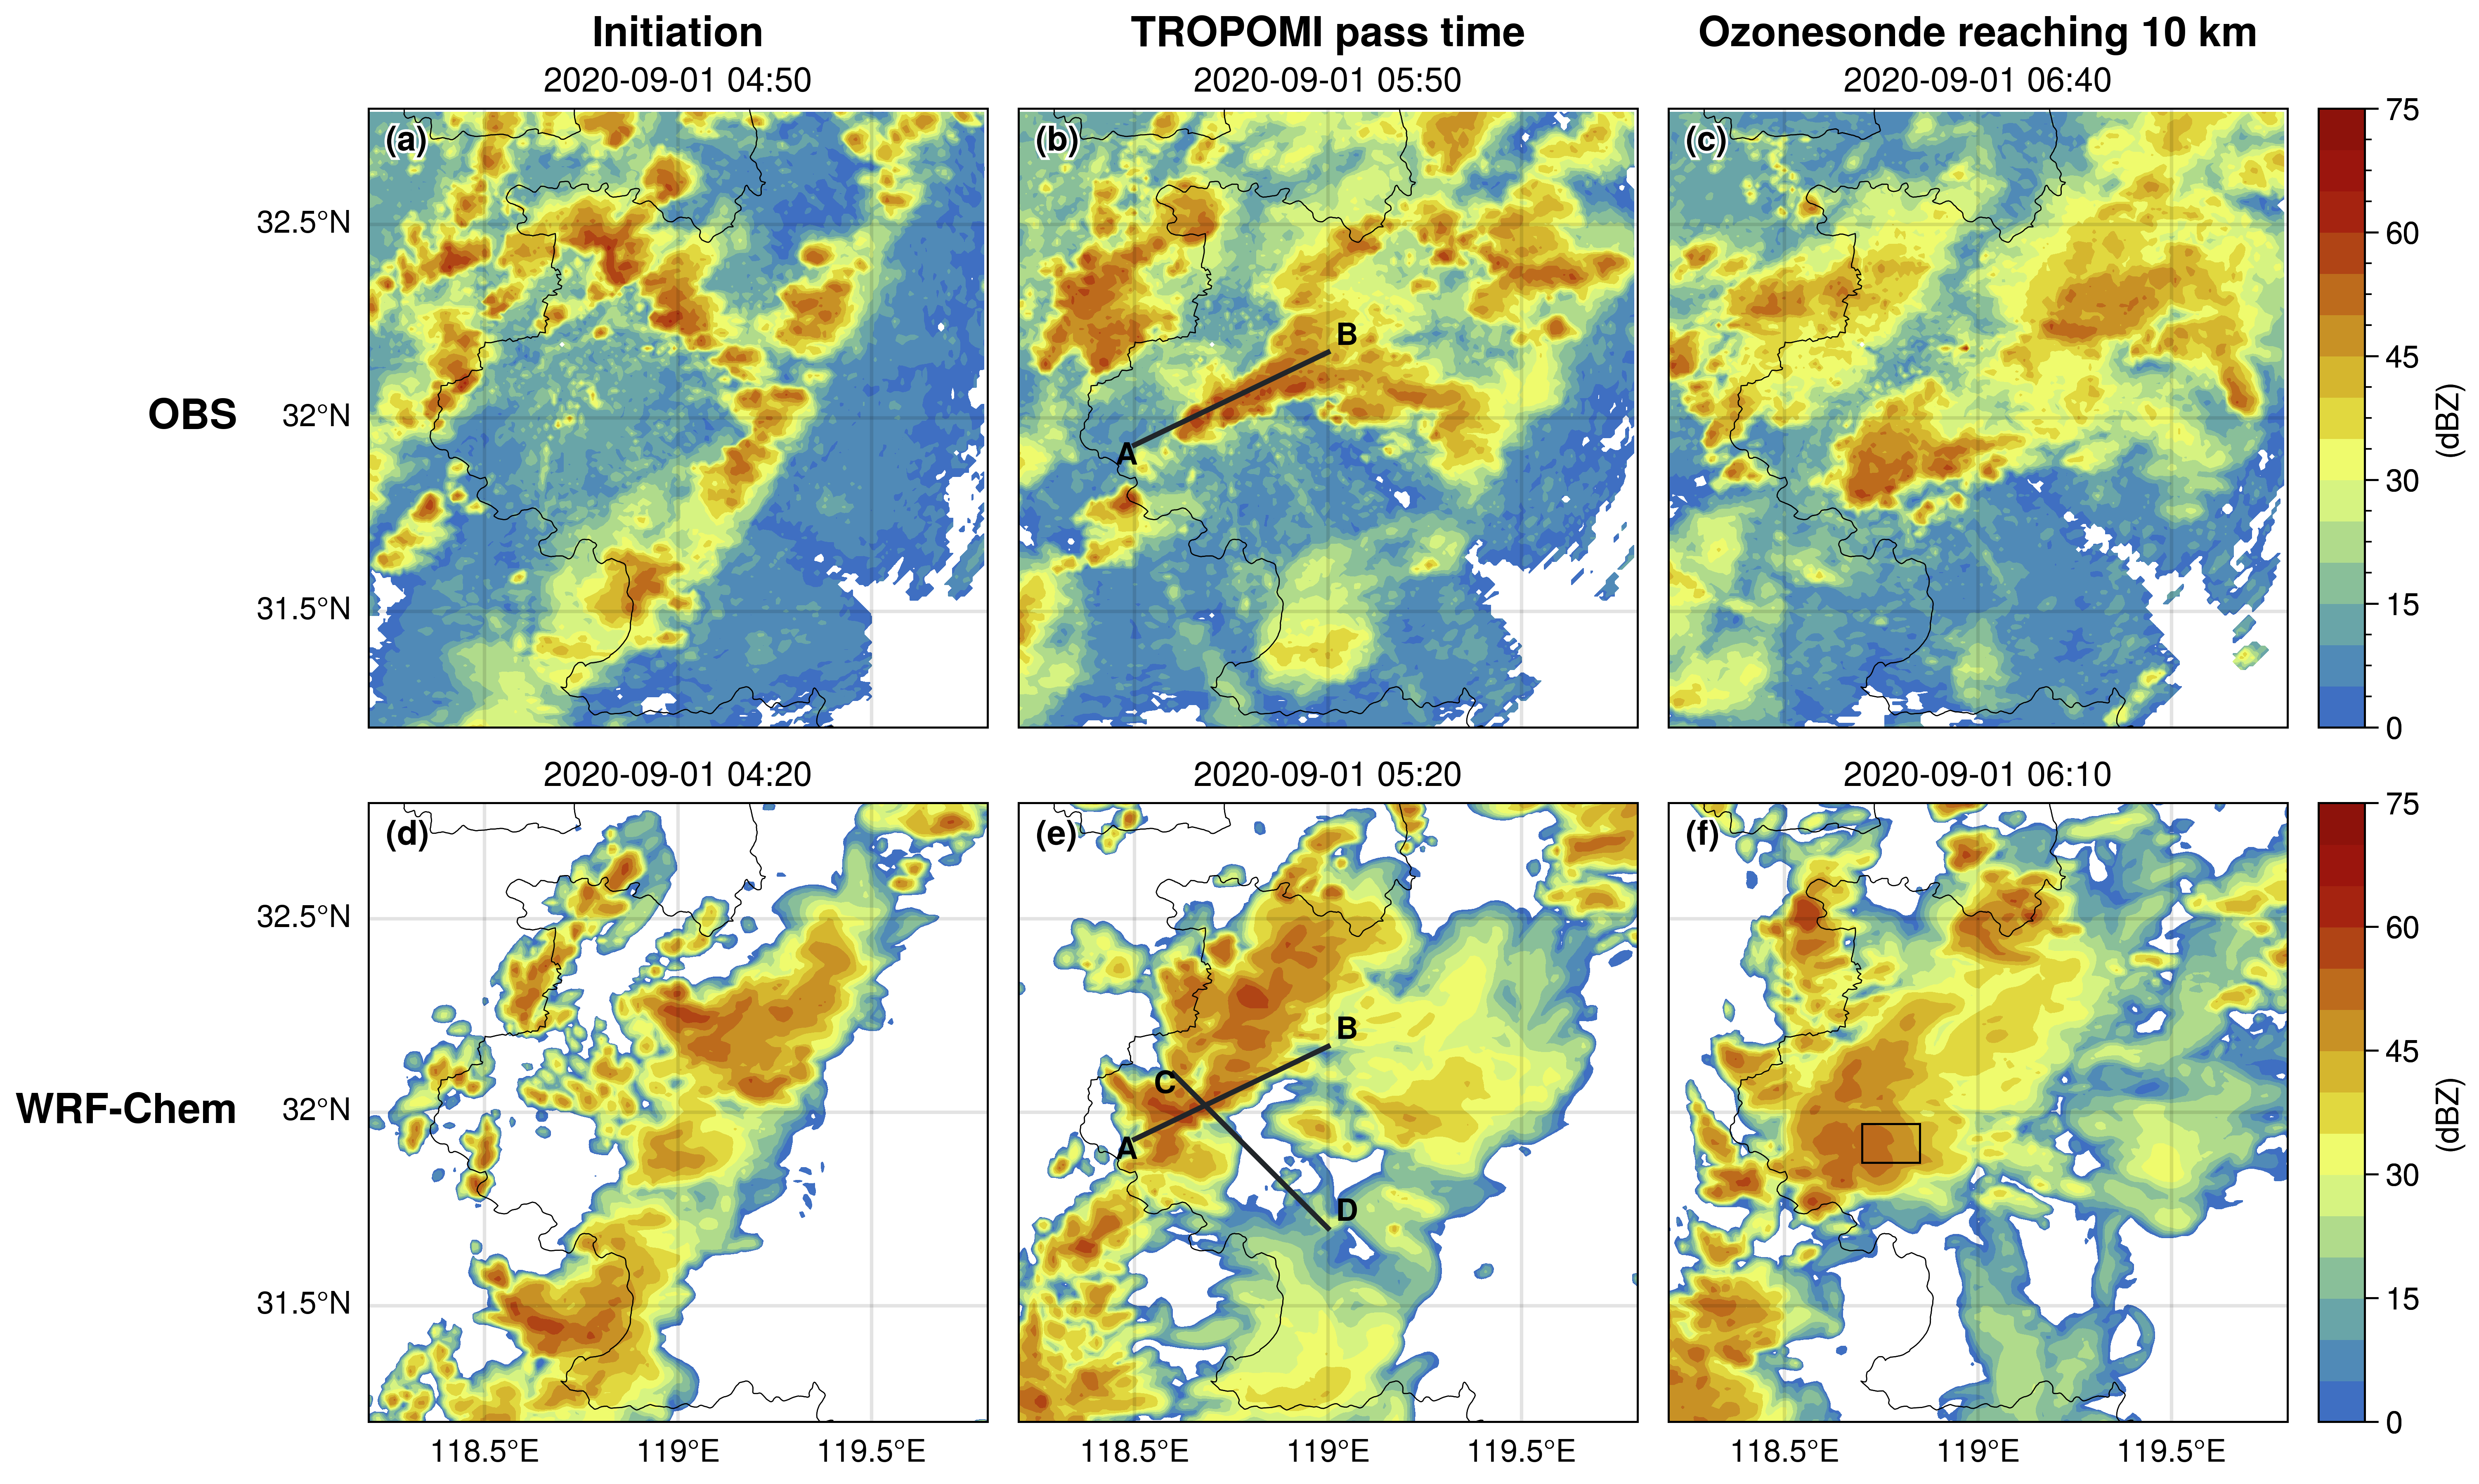
\includegraphics[width=0.9\textwidth]{./figures/comp_crf_2020.png}
\caption{与图\ref{fig:comp_crf_2019} 相同,但针对2020年9月1日的对流个例,模拟时间比雷达观测提前30分钟。\\
Figure \ref{fig:comp_crf_2020} Same as Fig. \ref{fig:comp_crf_2019} but for the case on 01 September 2020.
The simulation time is 30 minutes ahead of each radar observation.}
\label{fig:comp_crf_2020}
\end{figure}

\begin{figure}[htbp]
\centering
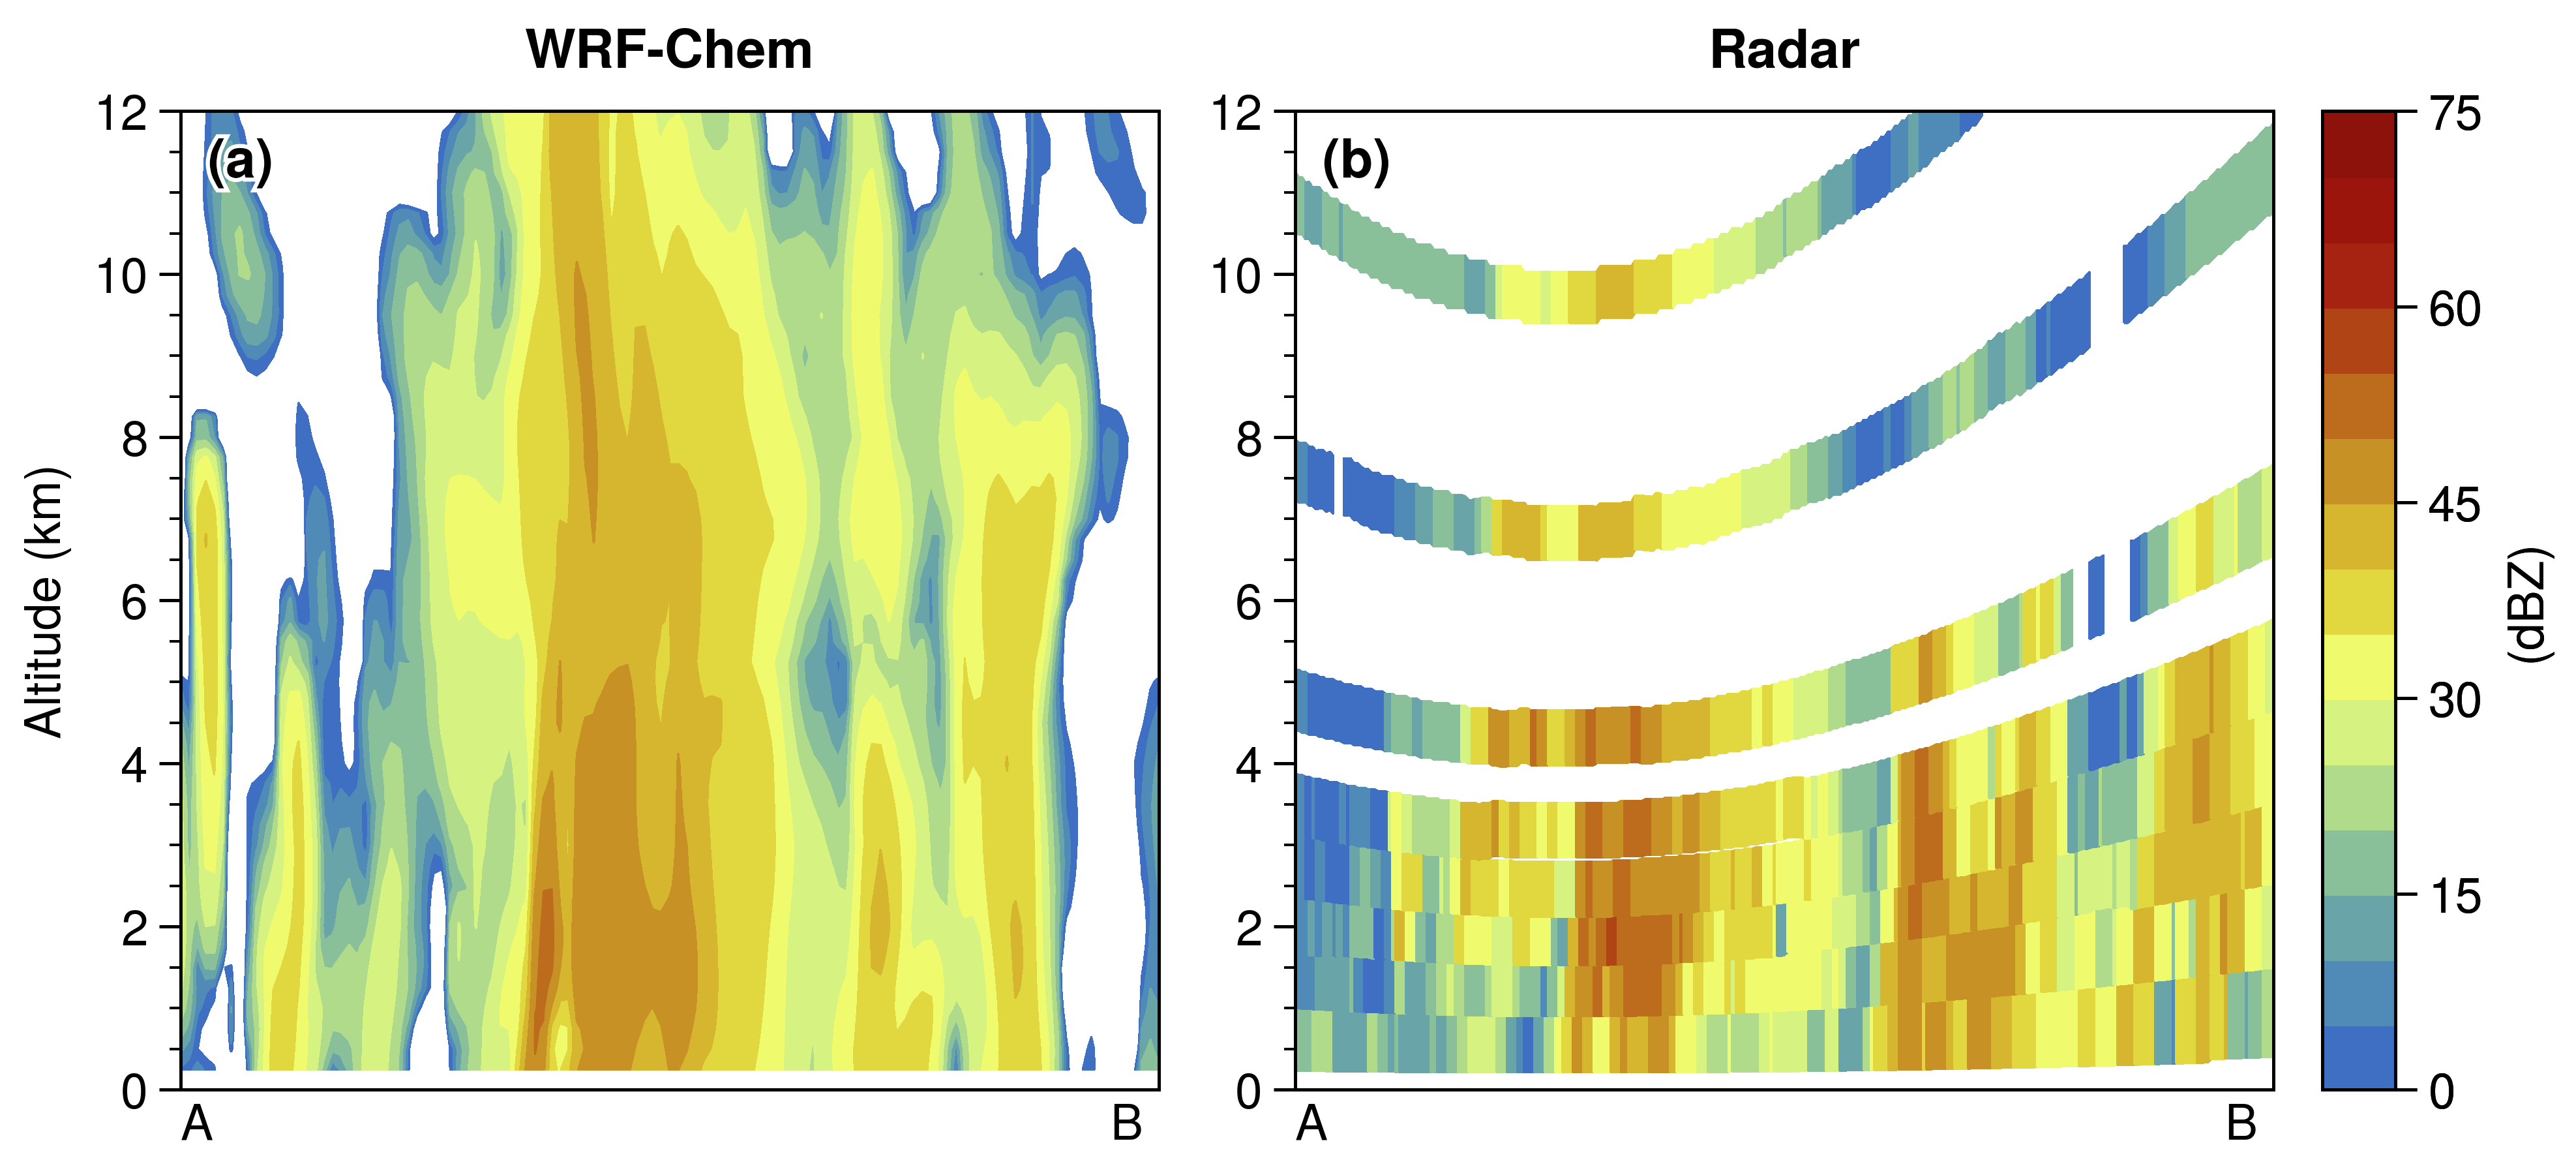
\includegraphics[width=0.8\textwidth]{./figures/comp_dbzcross_2019.png}
\caption{沿着图\ref{fig:comp_crf_2019}中AB线剖得的2019年7月25日(a)WRF-Chem模拟的和(b)雷达观测的雷达反射率。\\
Figure \ref{fig:comp_dbzcross_2019} Vertical cross sections of (a) WRF-Chem simulated and (b) observed radar reflectivity fields along the transect lines (AB) in Fig. \ref{fig:comp_crf_2019} for 25 July, 2019.}
\label{fig:comp_dbzcross_2019}
\end{figure}

\begin{figure}[htbp]
\centering
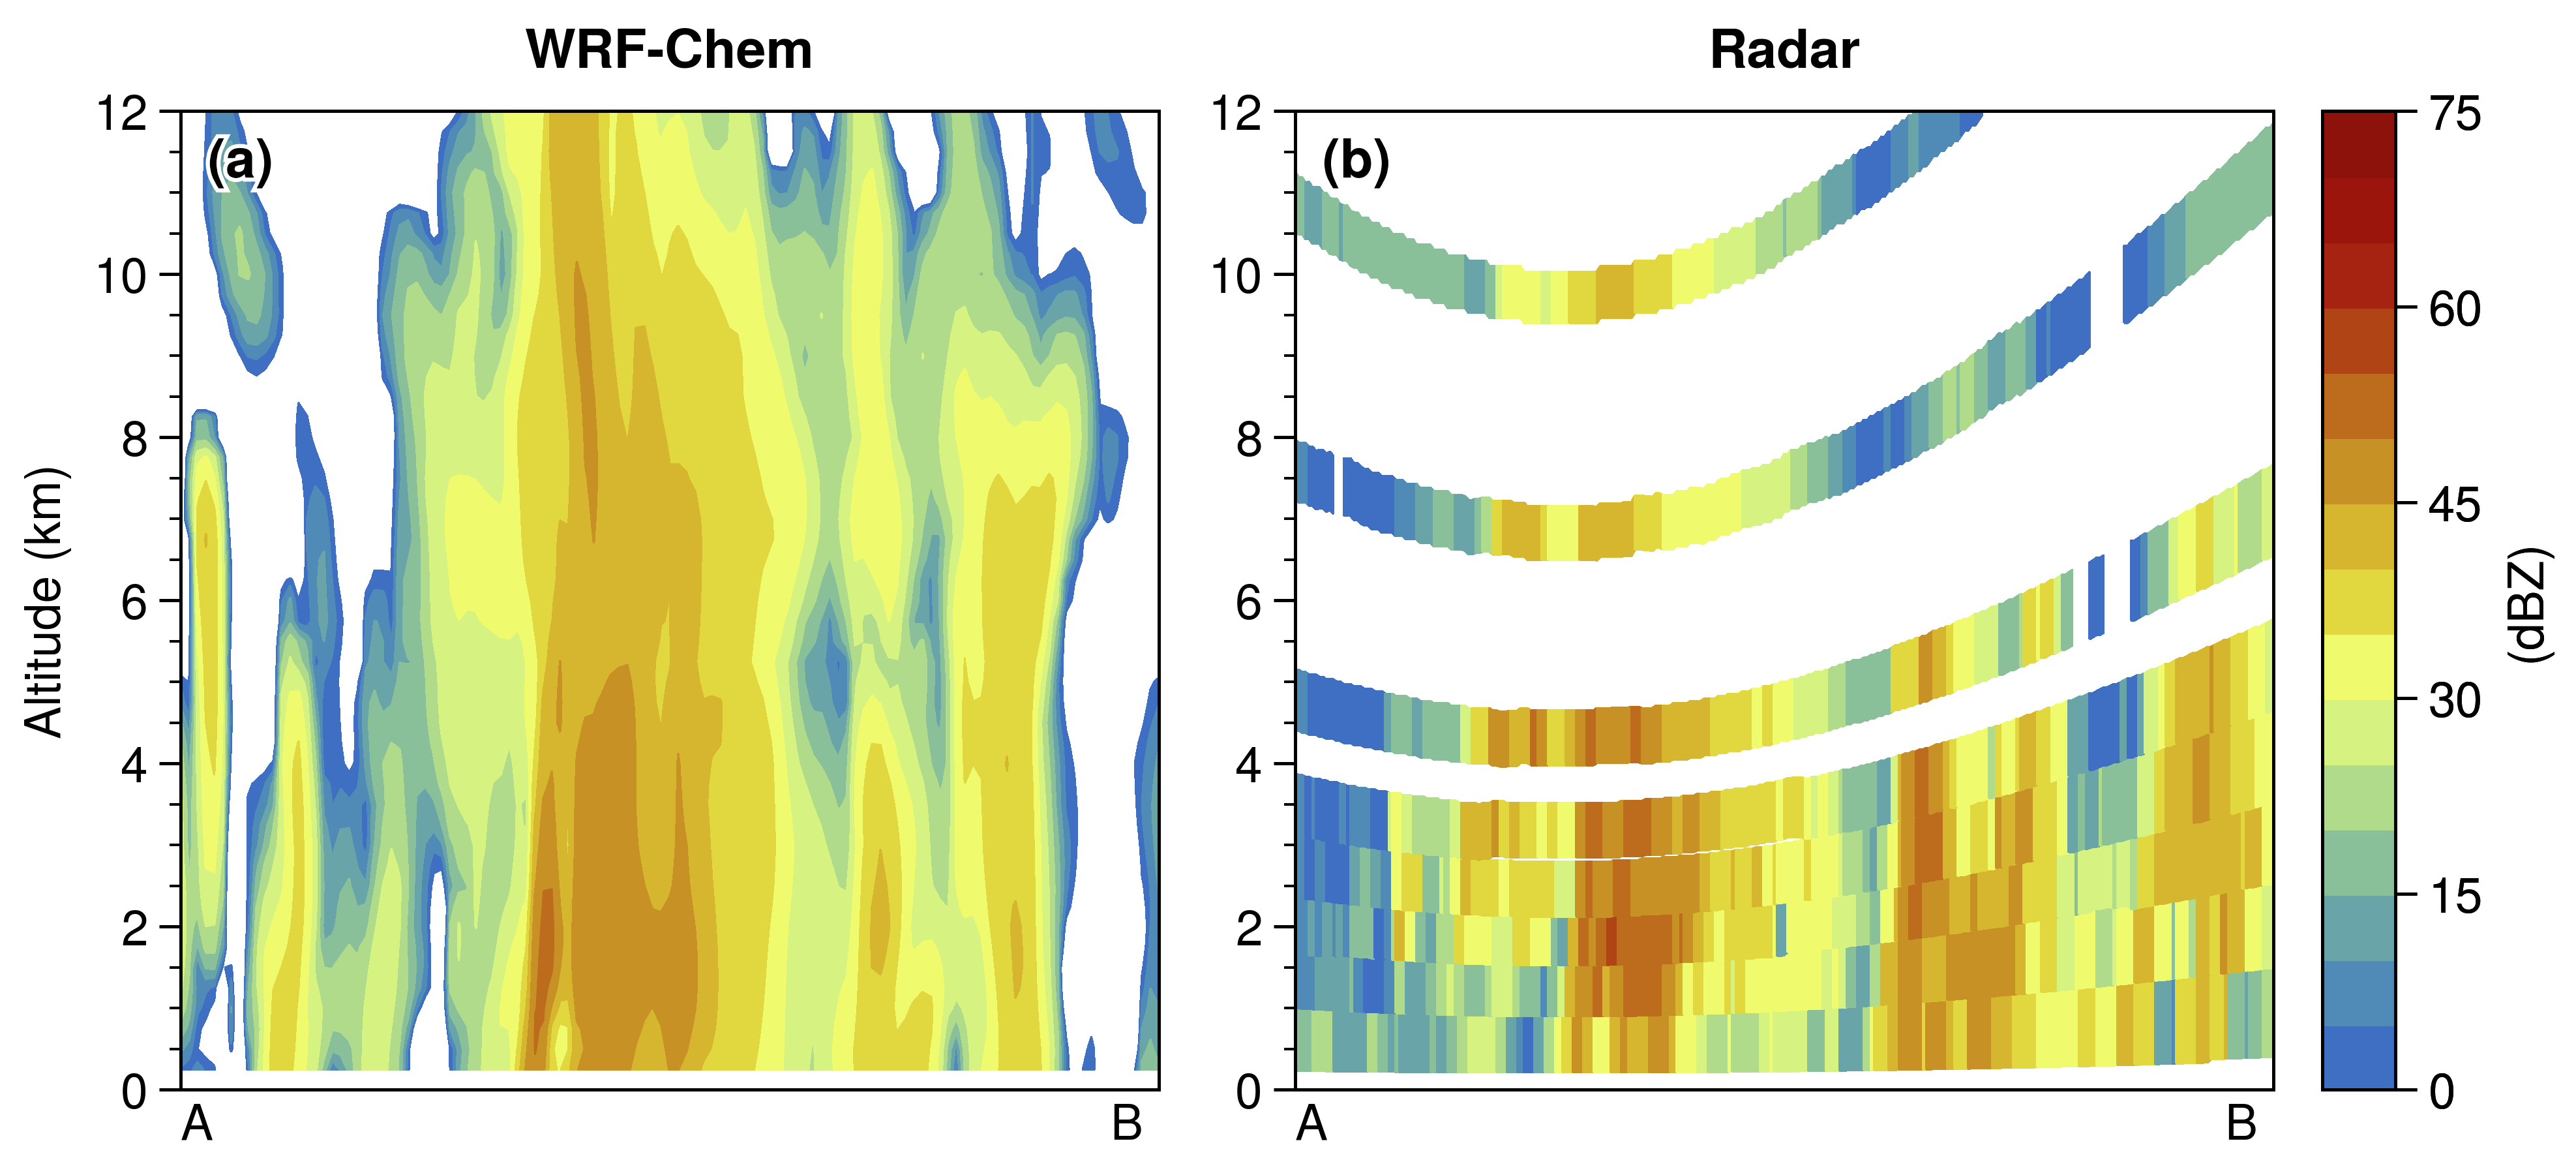
\includegraphics[width=0.8\textwidth]{./figures/comp_dbzcross_2019.png}
\caption{与图\ref{fig:comp_dbzcross_2019}相同,但针对2020年9月1日的对流个例。\\
Figure \ref{fig:comp_dbzcross_2020} Same as Figure \ref{fig:comp_dbzcross_2019} but for the case on 01 September 2020.}
\label{fig:comp_dbzcross_2020}
\end{figure}


\begin{figure}[htbp]
\centering
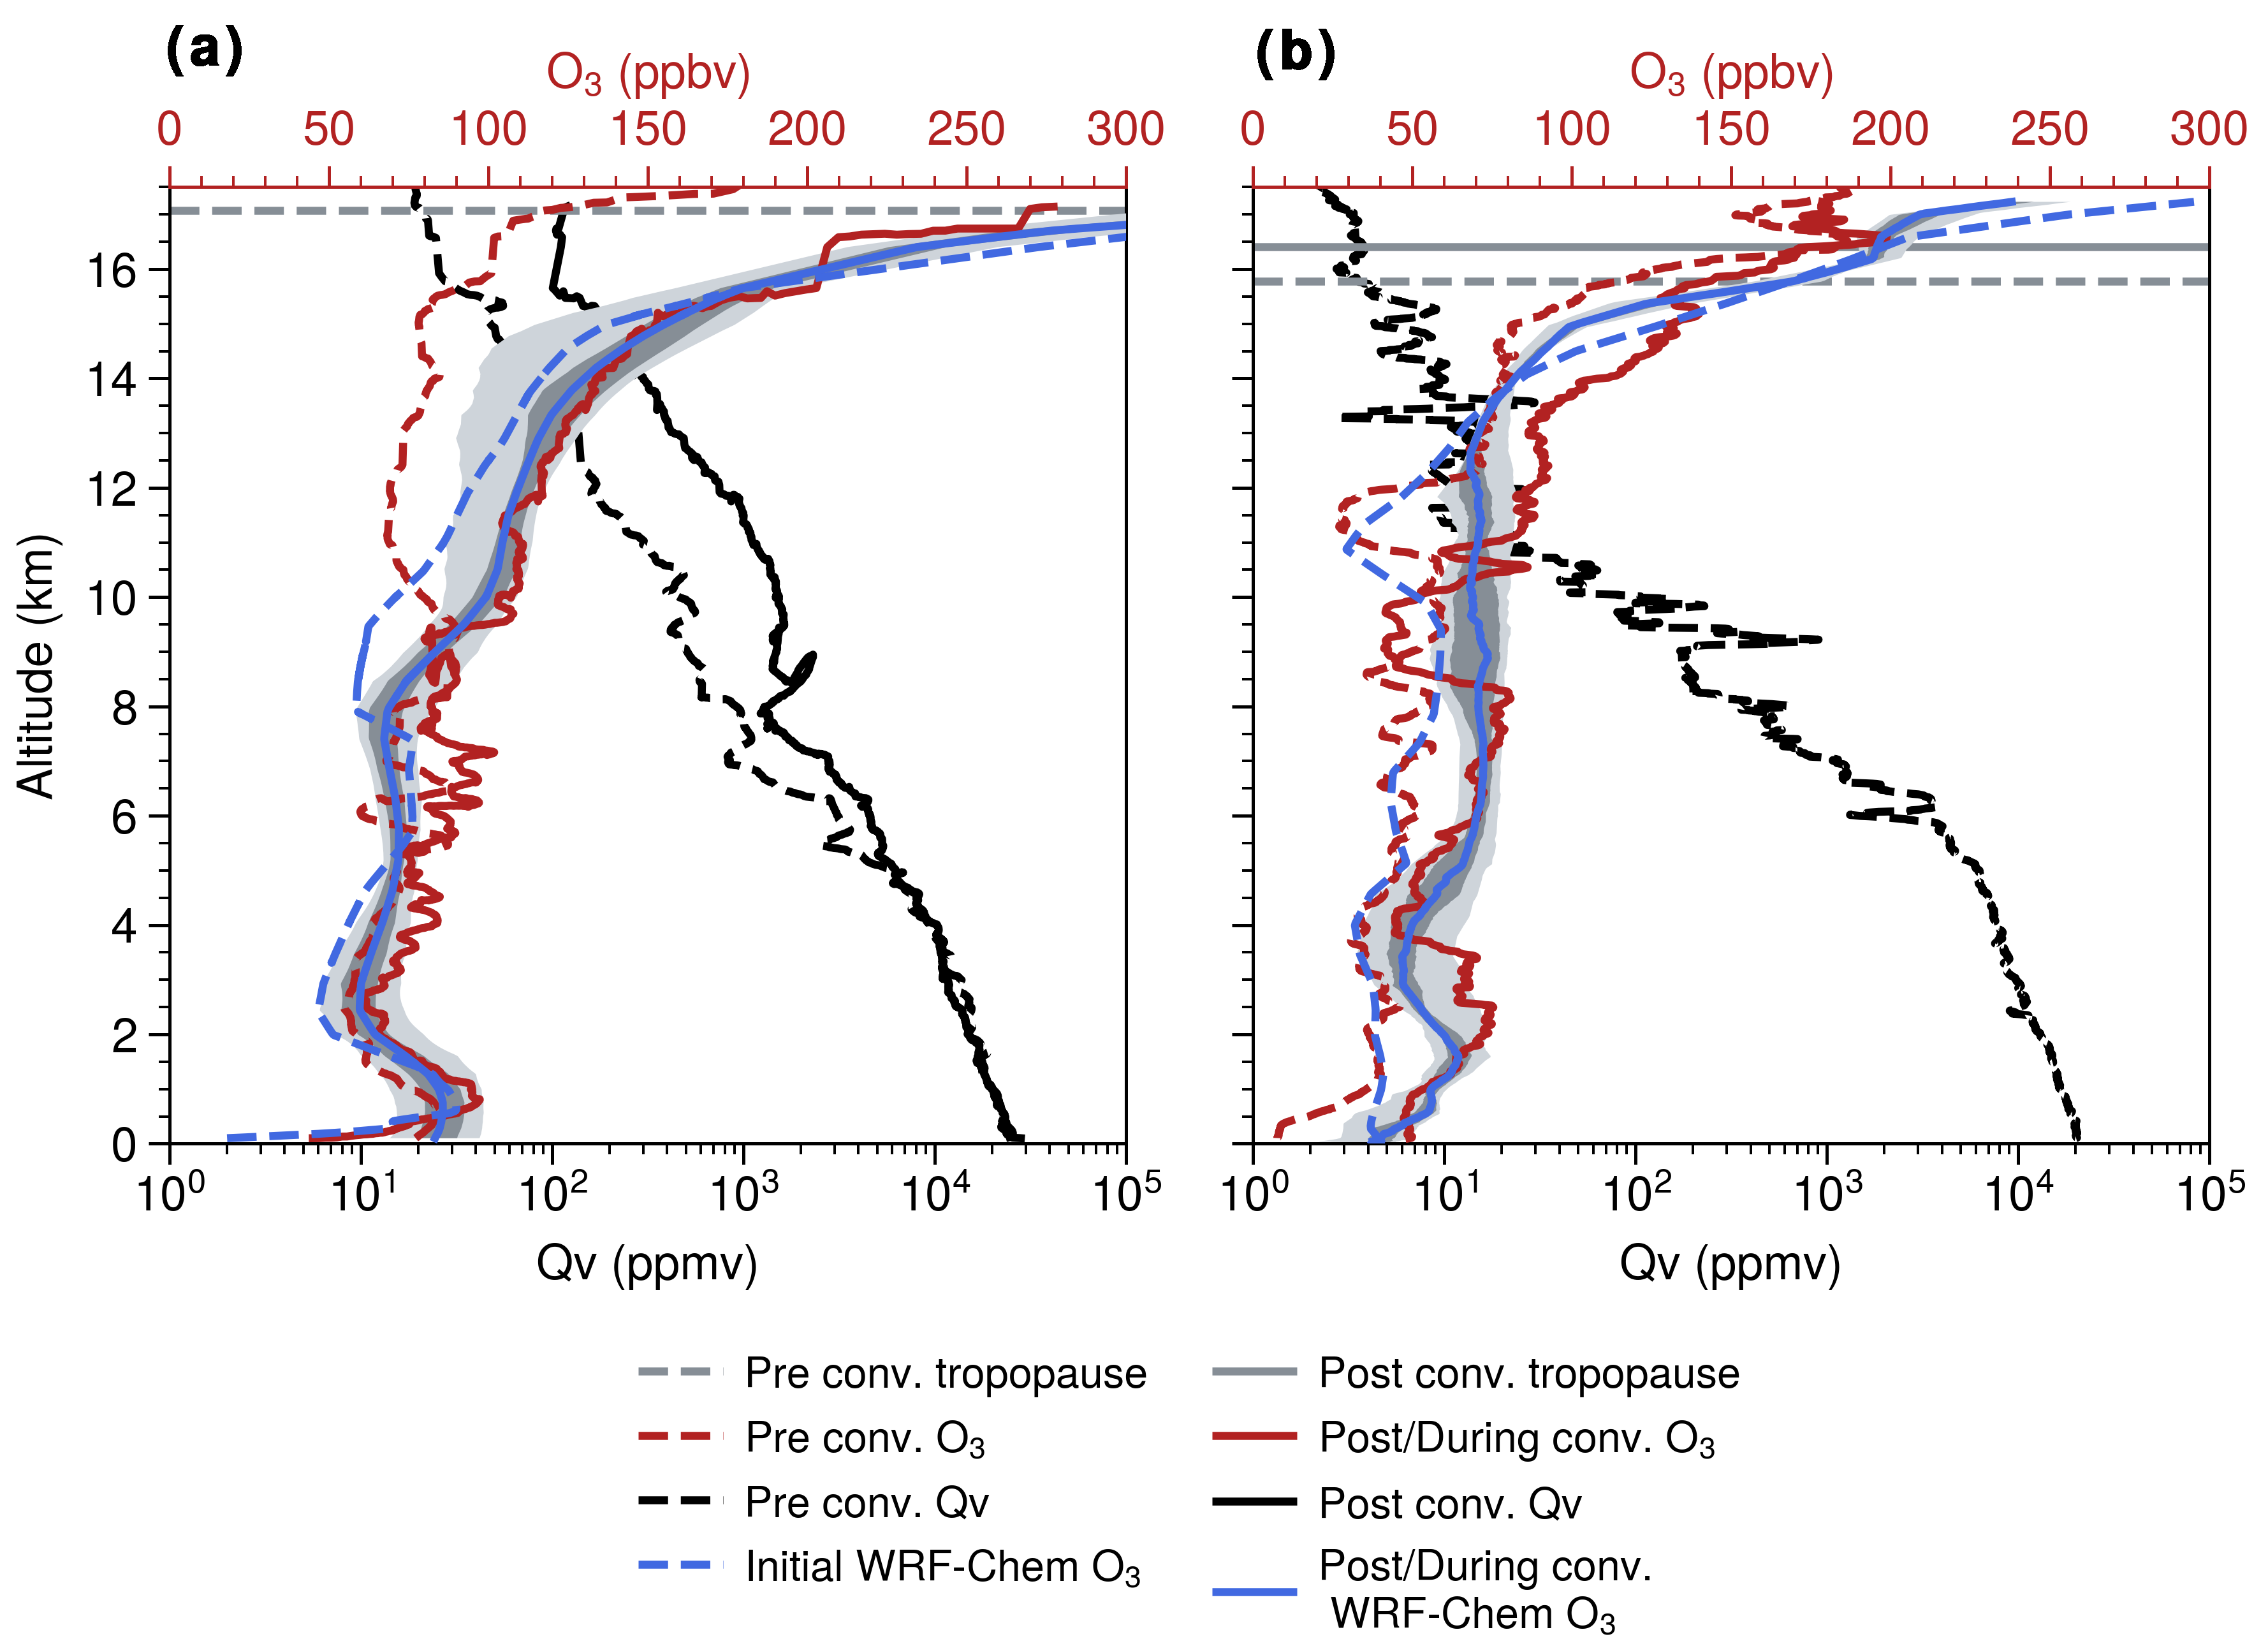
\includegraphics[width=0.8\textwidth]{./figures/ozonesonde_profile.png}
\caption{对流前(虚线)和对流后/对流期间(实线)探空观测到的O$_3$(红色)和Q$_v$(黑色)廓线。
模式初始(虚线)和对流后或对流期间(实线)的O$_3$廓线为蓝色。
深灰色阴影是50\%的置信区间,浅色是90\%的置信区间,灰线是第一对流层顶。\\
Figure \ref{fig:ozonesonde_profile} Observed O$_3$ (red) and Qv (black) profiles in the pre-convection (dashed) and post-convection/during-convection (solid) periods.
The initial (dashed) and simulated post-convection or during-convection (solid) O$_3$ profiles are in blue.
The dark gray shading is the 50 \% confidence interval while the light one is the 90 \% confidence interval.
The gray lines are the lapse rate tropopauses.
}
\label{fig:ozonesonde_profile}
\end{figure}




\section{结果与讨论}

\subsection{动力输送和化学反应对臭氧变化的贡献}




\begin{figure}[htbp]
\centering
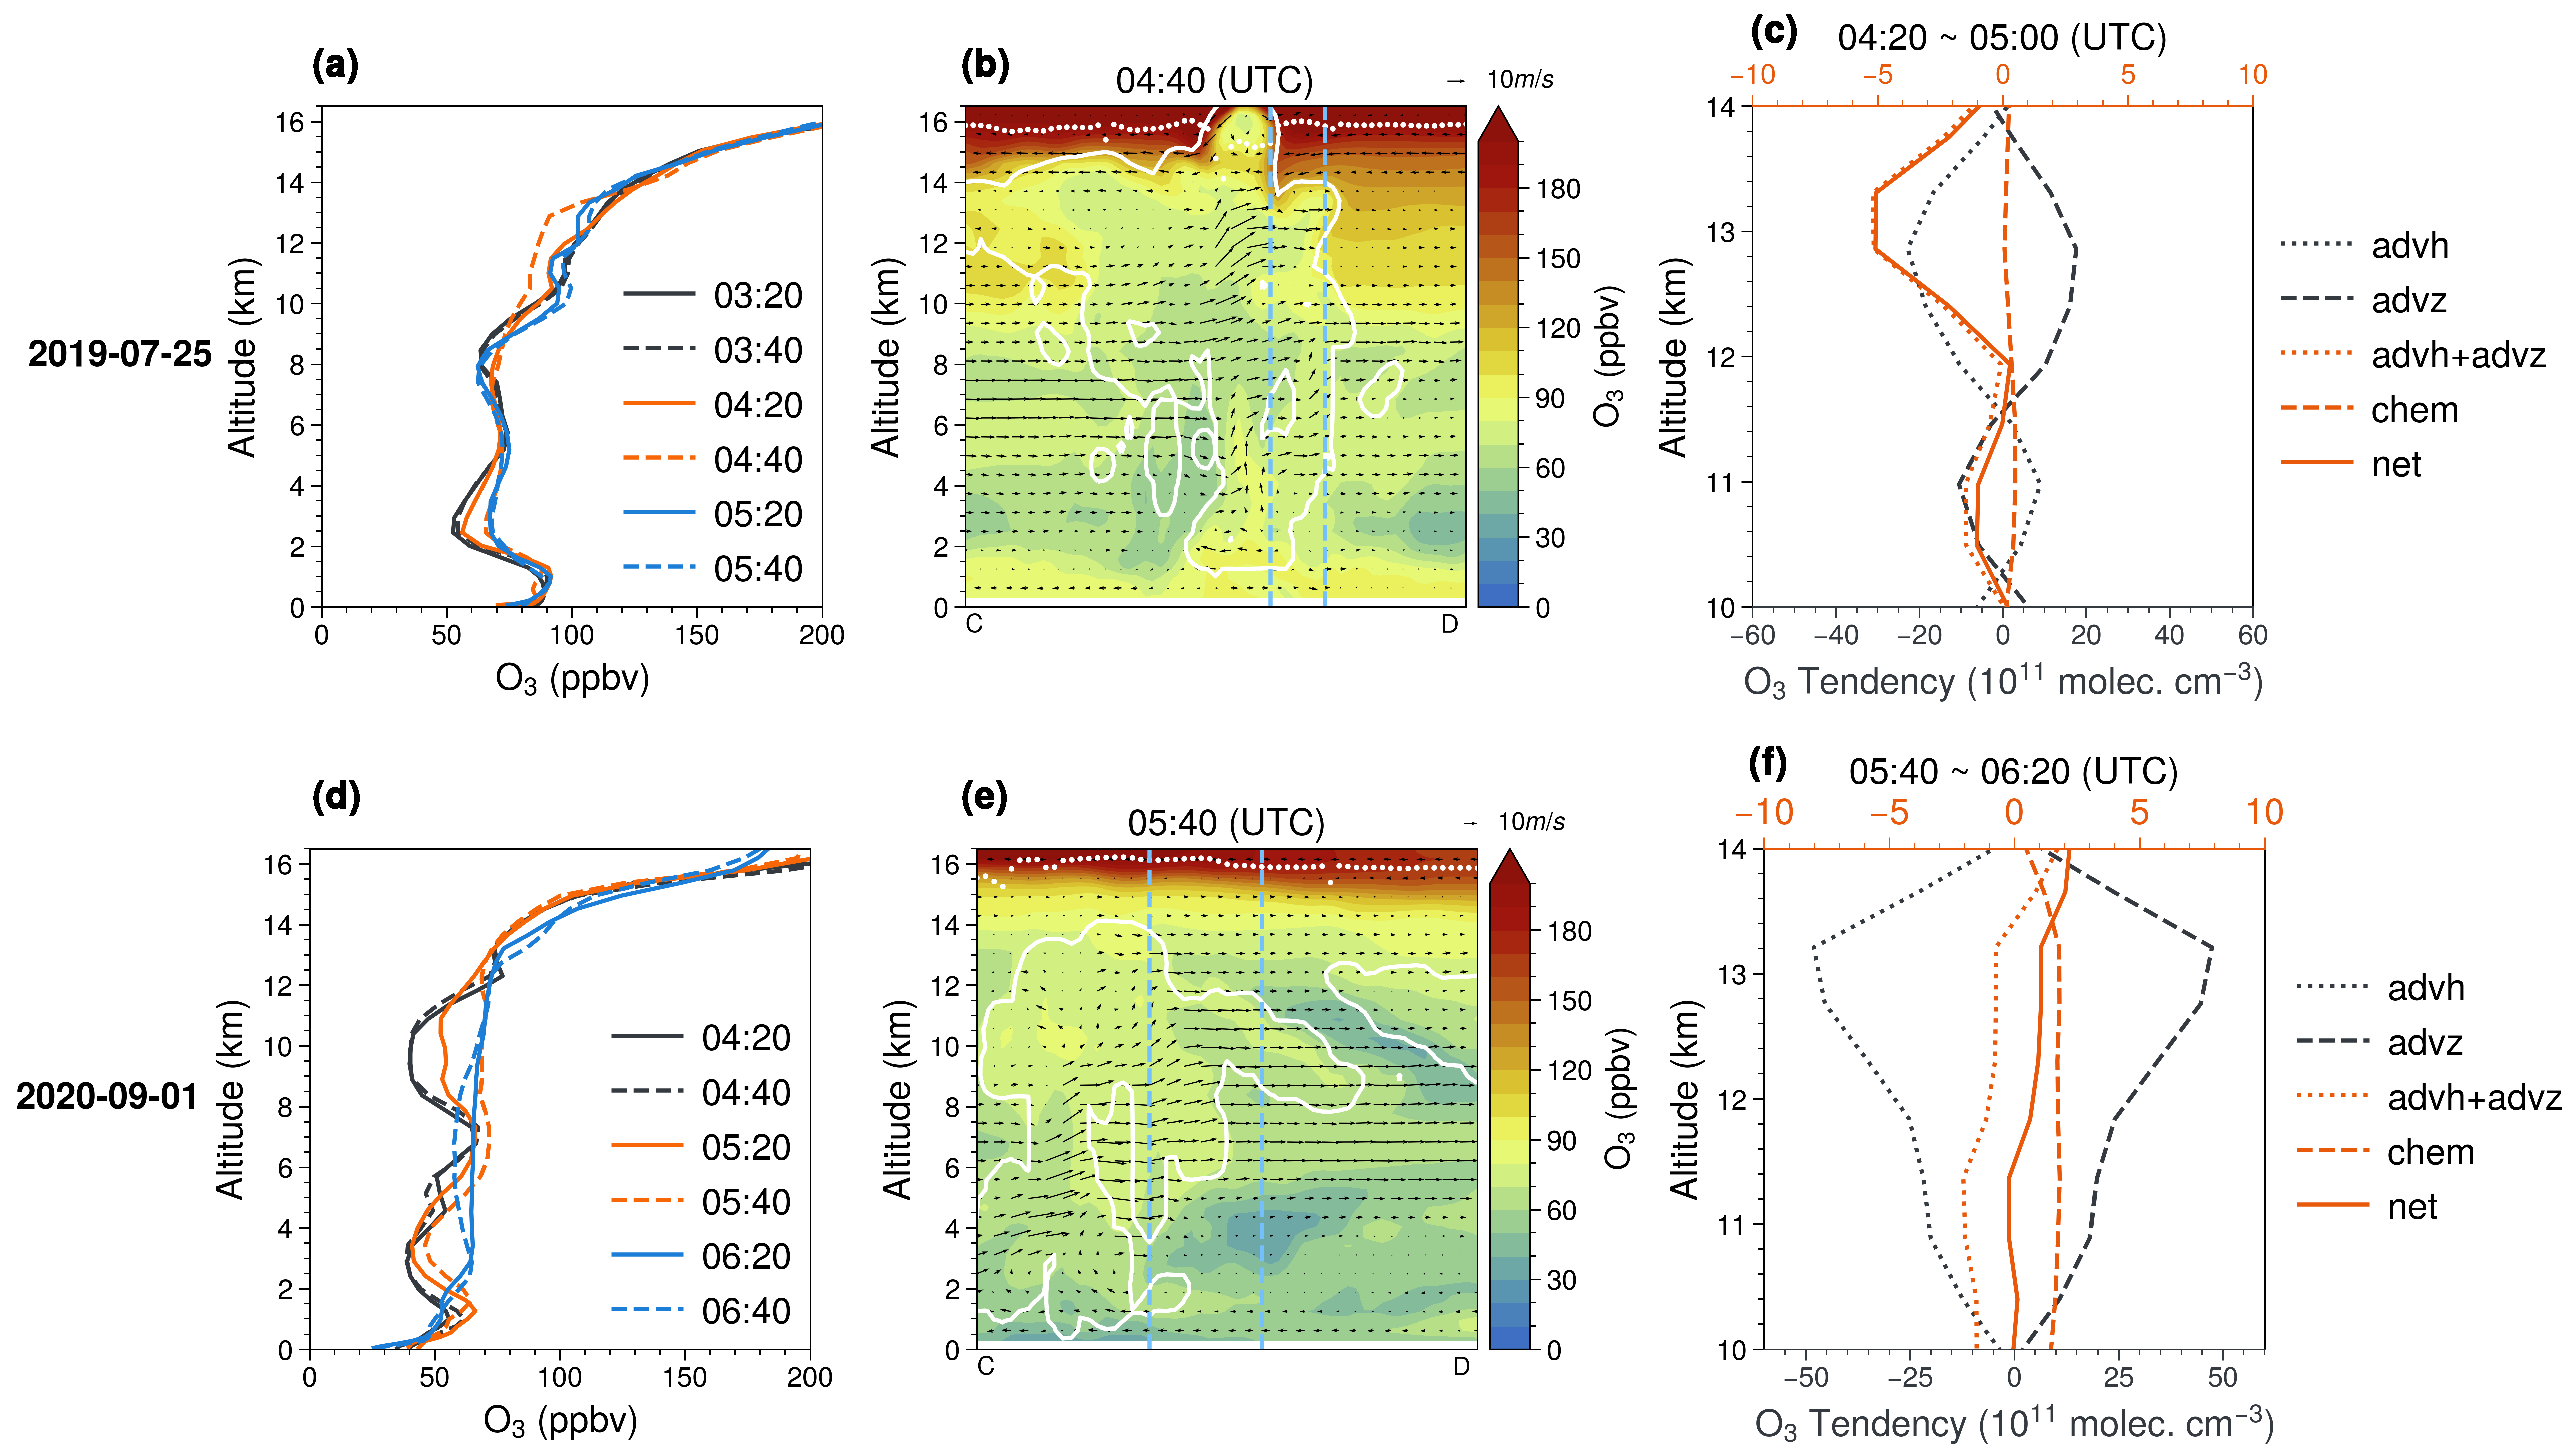
\includegraphics[width=\textwidth]{./figures/tendency_o3.png}
\caption{
(a, d) 臭氧探空仪经过区域的O$_3$平均浓度剖面,包括三个阶段:初生(黑色)、发展(橙色)和消散(蓝色)。
(b,e)对流旺盛期内沿穿过对流核心(图 \ref{fig:comp_crf_2019}e 和图 \ref{fig:comp_crf_2020}f)的O$_3$剖面。
蓝色虚线代表臭氧探空仪经过区域的边界,第一对流层顶显示为白点。
白线为云边界(云液态水混合比[q$_{cloud}$]和冰混合比[q$_{ice}$]之和 $\geq$ 0.01 g/kg)。
(c, f) 对流旺盛期的水平平流 (advh)、垂直平流 (advz) 和化学贡献 (chem)引起的O$_3$净生产率和趋势的垂直分布。
\\
Figure \ref{fig:tendency_o3} (a, d) The mean O$_3$ profiles in the regions passed by the ozonesondes
at three stages: initiation (black), development (orange), and dissipation (blue).
(b, e) Vertical O$_3$ distribution within the convective periods along the line crossing the convective core (Fig. \ref{fig:comp_crf_2019}e and Fig. \ref{fig:comp_crf_2020}f).
The blue dashed lines stand for the boundaries of regions passed by the ozonesondes, and the lapse rate tropopause is shown as the white dots.
The cloud boundaries (the sum of cloud liquid water mixing ratio [q$_{cloud}$] and ice mixing ratio [q$_{ice}$] $\geq$ 0.01 g/kg) are shown in white lines.
(c, f) The vertical distributions of the O$_3$ net production rate and tendency due to horizontal advection (advh), vertical (advz) advection, and chemistry (chem) during the convective periods.
}
\label{fig:tendency_o3}
\end{figure}




\subsection{闪电氮氧化物的影响}

\section{本章小结}
